\documentclass[11pt]{article}
\usepackage[a4paper,margin=22mm]{geometry}
\usepackage[T1]{fontenc}
\usepackage[utf8]{inputenc}
\usepackage{amsmath,amssymb,amsthm,mathtools,booktabs,array,graphicx,hyperref}

\usepackage[numbers,sort&compress]{natbib}
\hypersetup{hidelinks,pdftitle={Technical Companion: Annual Restriction Accounting for Non-Firm Transmission Access},pdfauthor={Alban Kryeziu, Stuart X. Zhu, Tolga Karabas, Evrim Ursavas}}
\newtheorem{proposition}{Proposition}
\newtheorem{lemma}{Lemma}
\newtheorem{theorem}{Theorem}
\newtheorem{remark}{Remark}
\newcommand{\pp}[1]{[#1]_+}
\newcommand{\one}{\mathbf1}
\newcommand{\R}{\mathbb R}
\newcommand{\F}{\mathcal F}
\title{Technical Companion: Annual Restriction Accounting for Non-Firm Transmission Access}
\author{Alban Kryeziu, Stuart X. Zhu, Tolga Karabas, and Evrim Ursavas\thanks{Department of Operations, Faculty of Economics and Business, University of Groningen, 9747 AE Groningen, The Netherlands. Corresponding author: a.kryeziu@rug.nl.}}
\date{17 October 2026 --- Version 1.0 (pre-deposit technical report)}
\begin{document}
\maketitle
\begin{abstract}
This standalone report accompanies Annual Restriction Accounting for Non-Firm Transmission Access: Entitlement Geometry and Network Effects. It provides exact debit-projection proofs, supporting-plane dual formulas, independently reconstructed guarded annual bounds, and physical-model diagnostics. Complete new multipliers are retained separately; the calculations are not outward-rounded interval certificates. Stored-array actuator floors are distinguished from unevaluated premium alternating-current and forecast-vintage extensions. Lower thermal residual under different debit rules is not an equal-protection or security result. The report is prepared for independent Zenodo deposit; no report DOI has yet been verified.
\end{abstract}
\section{The physical and contractual domain}
For position $n$ and hour $t$, let $P_n>0$, $v_{nt}\geq0$, $\chi_{nt}\leq\kappa_{nt}\in\{0,1\}$, $b_{nt}=\chi_{nt}\min\{P_n,v_{nt}\}$, $0\leq x_{nt}\leq b_{nt}$, and $z_{nt}=x_{nt}/P_n$. Set $H_n=\Delta\lfloor\rho\sum_t\kappa_{nt}\rfloor$ on the uniform grid. Each rule defines $\F^M=\{x:0\leq x\leq b,\ D_n^M(x)\leq H_n\ \forall n\}$, with support variables where needed.

For a fixed balanced mapping $\one^\top A=0$, let $p_t^{\rm req}=p_t^{\rm bg}-Av_t$ and $p_t(x_t)=p_t^{\rm req}+Ax_t$. A monitored row has $f_{jt}(x_t)=f_{jt}^{\rm req}+g_j^\top x_t$ and rating $F_j>0$. The objectives are $S(x)=\sum_t\Delta_t\sum_j[|f_{jt}(x_t)|-F_j]_+$ and $E_n(x)=\sum_t\Delta_tx_{nt}$. Soft thermal limits make zero action algebraically feasible. Balance alone does not guarantee feasible generator movements.

\section{Geometry of debit accounting}
Touched duration (M1), ordinary physical depth (M2), and hybrid debit are
\begin{align}
 \ell_{nt}u_{nt}\leq x_{nt}\leq b_{nt}u_{nt},\quad&u_{nt}\in\{0,1\},\quad\sum_t\Delta_tu_{nt}\leq H_n,\label{eq:support}\\
 D_n^2(x)=&\sum_t\Delta_t x_{nt}/P_n\leq H_n,\label{eq:m2}\\
 D_n^{H_\alpha}(x,u)=&\sum_t\Delta_t[\alpha u_{nt}+(1-\alpha)x_{nt}/P_n]\leq H_n.\label{eq:hybrid}
\end{align}
Here $0\leq\ell_{nt}\leq b_{nt}$; at $\alpha=0$ the support constraints are removed to recover M2 exactly. The request-normalized continuous interpolation is
\begin{equation}
 D_n^{R_\beta}(x)=\sum_{t:b_{nt}>0}\Delta_tx_{nt}\left[\frac{1-\beta}{b_{nt}}+\frac{\beta}{P_n}\right]\leq H_n.
 \label{eq:request}
\end{equation}
\begin{proposition}[Exact hybrid projection]
For $\alpha\in[0,1]$, the projection of \eqref{eq:hybrid} with $u_{nt}\in[0,1]$ and the relaxed support links is exactly $\F^{R_{1-\alpha}}$.
\end{proposition}
\begin{proof}
At $b_{nt}>0$, every relaxed lift satisfies $u_{nt}\geq x_{nt}/b_{nt}$. The least admissible activation $u_{nt}=x_{nt}/b_{nt}$ also satisfies $\ell_{nt}u_{nt}\leq x_{nt}$ and $u_{nt}\leq1$. Because the hybrid debit is nondecreasing in each $u_{nt}$, a lift exists if and only if its least-activation choice fits the budget. Substitution yields \eqref{eq:request} with $\beta=1-\alpha$. Zero-bound coordinates have $x_{nt}=u_{nt}=0$ without loss of generality.
\end{proof}
The threshold $\ell$ disappears from the relaxation. Even if every M1 positive action must satisfy $x\geq\ell$, the fractional activation $u=x/b$ is admissible for arbitrarily small $x>0$.

\begin{proposition}[Isolated convex hull]
Assume equal positive interval durations and an integer $K=H_n/\Delta$. For one uncoupled position, the projection of the M1-LP factor is the convex hull of its M1 action set.
\end{proposition}
\begin{proof}
For positive-bound coordinates put $y_t=x_{nt}/b_{nt}$. The relaxed factor is $\{y\in[0,1]^T: \sum_t y_t\leq K\}$. Every vertex is binary: two fractional components permit a perturbation in opposite directions along a tight knapsack row, and a single fractional component cannot make an integer right-hand side tight. An integral vertex is the image of an M1 action that chooses either zero or the full bound $b_{nt}$ in each supported hour. Those actions meet the materiality threshold. The projection contains all M1 actions, so equality follows.
\end{proof}
Convex-hull equality does not imply equality of minima for a convex objective. For $b_1=b_2=P=2$, $K=1$, and $S=[1-x_1]_++[1-x_2]_+$, M1 has minimum one, whereas the relaxed feasible point $(x_1,x_2)=(1,1)$ has value zero.

Since $x_{nt}/P_n\leq x_{nt}/b_{nt}\leq u_{nt}$ on each feasible M1 action, the exact inclusions are
\begin{equation}
 \F^{\mathrm{M1}}\subseteq\F^{R_0}\subseteq\F^{\mathrm{M2}},\qquad
 \F^{\mathrm{M1}}\subseteq\F^{H_\alpha}\subseteq\F^{\mathrm{M2}}.
\end{equation}
The debit wedge $D_n^{R_0}(x)-D_n^2(x)=\sum_{t:b_{nt}>0}\Delta_tx_{nt}(1/b_{nt}-1/P_n)$ is nonnegative. An observed positive wedge quantifies different treatment of one fixed action, not a causal decomposition of the resulting optimal objective difference.

\paragraph{Variation-sensitive debit.}
A temporally coupled protection rule charges both physical depth and upward depth changes:
\begin{equation}
 D_n^{V_\eta}(z)=\sum_t\Delta_tz_{nt}+\eta h_0\sum_t(z_{nt}-z_{n,t-1})_+,
 \qquad z_{n0}=0,\ \eta h_0\geq0.
 \label{eq:variation}
\end{equation}
Here $h_0$ has units of hours and $\eta\geq0$ is dimensionless. Unlike M2 and positive fixed-weight debit, this rule is not generally componentwise nondecreasing: reducing a restriction at time $t$ can create an additional upward change at $t+1$. Its debit still dominates ordinary FDE.

\section{The annual separation and the precision of its use}
Let $S^M=\inf\{S(x):x\in\F^M\}$. Let $L^{1L}$ be any valid lower bound on $S^{R_0}$, and let $x^2\in\F^{\mathrm{M2}}$ satisfy $S(x^2)\leq U^2$.
\begin{theorem}[Annual dominance witness]
If $U^2+\delta<L^{1L}$ with $\delta\geq0$, every M1-feasible action $x^1$ has $S(x^1)>S(x^2)$. When $L^{1L}>0$,
\begin{equation}
\frac{S(x^1)-S(x^2)}{S(x^1)}\geq 1-\frac{U^2+\delta}{L^{1L}}>0.
\end{equation}
\end{theorem}
\begin{proof}
$S(x^2)\leq U^2\leq U^2+\delta<L^{1L}\leq S^{R_0}\leq S(x^1)$. Dividing the inequality $S(x^2)\leq U^2+\delta$ by $S(x^1)\geq L^{1L}>0$ gives the stated relative result.
\end{proof}
The theorem is exact. The numerical evaluation uses independently reconstructed full-box restricted masters and the original B03 feasible M2 witnesses. All new multipliers are retained; signs and hourly sums are independently checked, followed by finite-box reconstruction and coefficient/accumulation guards. Exact rational checks establish feasibility of the stored witness coordinates. This remains guarded floating-point evidence, not fully outward-rounded interval arithmetic. In the Dutch evaluation, the guarded pairs $(U^2,L^{1L})$ in millions of residual units are $(48.058421891,57.909827749)$, $(32.237842053,37.782287250)$, and $(18.740819468,23.658821383)$ for 2029--2031. The corresponding full-precision relative margins are 17.0116\%, 14.6747\%, and 20.7872\%. Displayed endpoints are rounded outward; percentages use unrounded records.

\section{Network-relief scores and conservative rate cards}
With $\psi_t(x_t)=\sum_j[|f_{jt}^{\rm req}+g_j^\top x_t|-F_j]_+$, the one-sided coordinate benefit at the zero restriction is $m_{nt}=-P_n\psi_t'(0;e_n)$ when $b_{nt}>0$. Its full boundary-aware formula is
\begin{align}
 m_{nt}=-P_n\bigg(&\sum_{j:f_{jt}^{\rm req}>F_j}g_{jn}-\sum_{j:f_{jt}^{\rm req}<-F_j}g_{jn}\notag\\
&+\sum_{j:f_{jt}^{\rm req}=F_j}[g_{jn}]_+
+\sum_{j:f_{jt}^{\rm req}=-F_j}[-g_{jn}]_+\bigg).
\end{align}
The two boundary contributions penalize marginally induced overloads. They are necessary because a maximum-of-affine representation is only directionally differentiable at its breakpoints. For a single row $f^{\rm req}=10.5$, $F=10$, $g=-1$, and $P=100$, the true right-derivative score is 100, whereas the 1-MW finite-step score is only 50. Hinge crossings therefore matter when interpreting scores.

Given exposure weights $w_{nty}=\Delta_t x_{nty}^{II}/P_n$ in fitting years, partition positive-weight observations by exposure-weighted relief-score tertiles. Let $W_b>0$ and $\bar m_b$ be bucket exposure and mean score. With $s=\max\{1,\max_b|\bar m_b|\}$, choose ordered $q_1\geq q_2\geq q_3$ by
\begin{align}
 \min_q\;&\sum_b W_b(\bar m_b/s)q_b+\frac\lambda2\sum_b W_b(q_b-\bar q)^2\notag\\
 \text{s.t. }\;&W^\top q=\bar q\sum_bW_b,\quad1\leq q_b\leq1+\gamma.\label{eq:card}
\end{align}
The uniform point $q=\bar q\one$ is feasible when $0\leq\xi\leq\gamma$ and $\bar q=1+\xi$. For $W_b>0,\lambda>0$ the minimizer is unique. If $0<\xi<\gamma$, $\bar m_1\leq\bar m_2\leq\bar m_3$, and $\bar m_1<\bar m_3$, the direction $(1/W_1,0,-1/W_3)$ is feasible locally at the uniform point and decreases the linear term. Thus the minimizer must be nonuniform.

A different signal $a_{nty}=\mu_{ny}w_{nty}$, with an annual Stage-II entitlement multiplier $\mu_{ny}$, measures a local secondary-energy sensitivity only if the primary residual cap is held fixed. If the cap $C_S(q)$ also varies, the complete value derivative additionally includes $-\eta\,\mathrm d C_S/\mathrm dq$ under regularity. Its aggregate ratios $A_b/W_b$ average position-year multipliers. The former fitting QP with mean one, the same order, and a positive quadratic ridge is forced to $q=\one$ if $A_1/W_1\geq A_2/W_2\geq A_3/W_3$. To see this, write $d=q-\one$ and use the weighted pairwise identity
\begin{equation}
 A^\top d=\frac{1}{\sum_bW_b}\sum_{i<j}W_iW_j\left(\frac{A_i}{W_i}-\frac{A_j}{W_j}\right)(d_i-d_j)\geq0.
\end{equation}
This condition applies to the selected $\rho=0.15$ ridge-import aggregates. Sparse export reference exposure triggers a fallback, while a separate nonuniform histogram candidate is rejected in validation. The condition does not apply to all candidates or directions and is not a universal failure of dual-based sensitivity methods.

\section{Safety of positive-premium rules and exposure witnesses}
For $D_n^q(x)=\sum_t\Delta_t q_{nt}x_{nt}/P_n$, any fixed $q_{nt}\geq1$ implies $D_n^q(x)\geq D_n^2(x)$ for all nonnegative $x$. Hence $\F^{C_q}\subseteq\F^{\mathrm{M2}}$ and the globally optimal annual M2 residual cannot be exceeded in quality by a conservative card. This inclusion compares exact annual optima and implies no ranking of two finite-horizon rolling outputs.

Let $x^C$ and $x^U$ be feasible annual output witnesses under $q^C\geq1$ and $q^U=\bar q\geq1$, respectively. Define $\alpha_n=\min\{1,E_n(x^U)/E_n(x^C)\}$ when $E_n(x^C)>0$, and $\alpha_n=1$ otherwise. Put $x^{EC}_{nt}=\alpha_nx^C_{nt}$. Nonnegative coefficients give
\begin{align}
 D_n^C(x^{EC})&\leq D_n^C(x^C)\leq H_n,\\
 D_n^U(x^{EC})&=\bar qE_n(x^{EC})/P_n\leq\bar qE_n(x^U)/P_n\leq H_n.
\end{align}
The physical box and soft thermal constraints are preserved. Therefore $x^{EC}$ is feasible in \emph{both} premium domains and uses no more restricted energy at any position than the uniform reference. An improvement in $S$ is a counterexample to local optimality of the stored uniform rolling schedule in the full annual domain, not evidence that uniform debit necessarily performs worse than a state-aware contract. The construction is retrospective and uses the complete final exposure of the uniform output.

\section{Screening, decomposition, and bound reconstruction}
The two signed hinge terms for every monitored row $j$ are
\begin{equation}
 \Delta_t[f_{jt}^{\rm req}-F_j+g_j^\top x_t]_+,
 \qquad\Delta_t[-f_{jt}^{\rm req}-F_j-g_j^\top x_t]_+.
\end{equation}
Writing all hour-$t$ hinges as $[a_{tj}^\top x_t+b_{tj}]_+$, their largest possible affine argument on $0\leq x_t\leq b_t$ is $b_{tj}+\sum_n\max\{0,a_{tjn}b_{nt}\}$. A hinge can be discarded if this number is nonpositive. After that elimination, a coordinate with $a_{tjn}\geq0$ in every retained hinge cannot decrease any overload term by increasing $x_{nt}$, so fixing it to zero is optimal when debit is componentwise nondecreasing and no other constraint requires positive $x_{nt}$. The physics sign is explicit: nonnegative coefficients mean that curtailment fails to relieve each potentially active directed overload. The operation is safe for M1, M2, and nonnegative-rate cards, with the corresponding support variable reset to zero if necessary.

\paragraph{Why variation debit changes screening.}
For three unit-duration hours take $\eta h_0=2$ and $z_0=0$. Under \eqref{eq:variation}, $z=(1,1,1)$ consumes $3+2=5$ hours, while decreasing only its middle component gives $z=(1,0,1)$ and consumes $2+2(2)=6$ hours. Thus the act of fixing a congestion-aggravating middle coordinate to zero can violate an annual variation-debit budget even though the restriction itself decreases. More generally, decreasing $z_t$ by $\epsilon$ reduces the physical term by $\Delta_t\epsilon$ and can increase the next upward-change penalty by at most $\eta h_0\epsilon$. Therefore $\eta h_0\leq\min_t\Delta_t$ is sufficient for componentwise monotonicity (including at boundary coordinates), and restores the debit requirement of the coordinate-screening proposition. It is not required for the hinge-removal test, which depends only on the physical box.

For an hourly hinge family $\mathcal J_t$, the exact identity
\begin{equation}
 \sum_{j\in\mathcal J_t}[a_{tj}^\top x_t+b_{tj}]_+
 =\max_{J\subseteq\mathcal J_t}\sum_{j\in J}(a_{tj}^\top x_t+b_{tj})
\end{equation}
permits one epigraph $\theta_t$ per hour and an initially small set of valid supporting inequalities. At a candidate $x_t$, adding the subset of strictly positive hinges gives a support tight at that candidate. Full-row re-evaluation is required before accepting a master objective or a secondary cap.

Let the post-screening annual LP master be $\min\{C_0+\sum_t\theta_t: Dx\leq H,\ 0\leq x\leq\bar x,\ a_{tk}^\top x+b_{tk}\leq\theta_t,\ \theta_t\geq0\}$. For any $\lambda\geq0$ and $\zeta_{tk}\geq0$ satisfying $\sum_k\zeta_{tk}\leq1$ for every hour, define $r=D^\top\lambda+\sum_{t,k}\zeta_{tk}a_{tk}$. Lagrangian minimization over the box yields the valid lower bound
\begin{equation}
 L_I=C_0-H^\top\lambda+\sum_{t,k}\zeta_{tk}b_{tk}+\sum_j\bar x_j\min\{r_j,0\}.
\end{equation}
For energy minimization with coefficients $e$ and cap $C_0+\sum_t\theta_t\leq C_S$, use a cap multiplier $\eta\geq0$ and $\sum_k\zeta_{tk}\leq\eta$. Then $r_{II}=e+D^\top\lambda+\sum\zeta a$, and
\begin{equation}
 L_{II}=-H^\top\lambda+\sum_{t,k}\zeta_{tk}b_{tk}+\eta(C_0-C_S)+\sum_j\bar x_j\min\{r_{II,j},0\}.
\end{equation}
The box correction is necessary without exact stationarity. Historical complete duals are missing; the new independent Stage-I certificates instead retain all $\lambda,\zeta$ and their support/row mappings. The full-box masters have 363,540, 420,480, and 468,660 columns and 82,799, 74,411, and 112,965 rows; no historical coordinate screening is imposed. They use all 8,760 hourly epigraphs and $C_0=0$. Solver-free support-column and physical-row reconstructions agree within numerical error. Downward guards are $9.42\times10^{-5}$, $2.93\times10^{-5}$, and $9.68\times10^{-6}$ residual units. Additional upper-replay error estimates below 0.0061 units do not close any separation. Complete interval enclosure was not performed.

\section{Analytical Diagnostics for Actuator Floors and Forecast Timing}
\subsection{Actuator-limited residual floor}
For every signed DC state-element row $j$ and hour $t$, the full independent physical box implies
\begin{align}
 \underline f_{jt}&=f_{jt}^{\rm req}+\sum_n\min\{0,g_{jn}b_{nt}\},\\
 \overline f_{jt}&=f_{jt}^{\rm req}+\sum_n\max\{0,g_{jn}b_{nt}\}.
\end{align}
The reachable flow is an interval containing the effect of every feasible annual action at that hour. Its smallest possible row exceedance is
\begin{equation}
 \underline s_{jt}=\max\{0,\underline f_{jt}-F_j,-F_j-\overline f_{jt}\}.
\end{equation}
Thus, for any annual feasible action,
\begin{equation}
 S(x)\geq\sum_t\Delta_t\sum_j\underline s_{jt},\qquad
 \max_{t,j}[|f_{jt}(x)|-F_j]_+\geq\max_{t,j}\underline s_{jt}.
\end{equation}
Temporal entitlement constraints only shrink the hourly boxes, so these lower bounds remain valid. They can be loose because different rows require conflicting actions. A separate stored-array audit evaluates the three annual-M2 peak row-hours: all occur on line 45 under outage of line 44. Table~\ref{tab:peakfloor} reports those box extrema, with no new optimizer.\begin{table}[ht]
\centering\small
\caption{Rowwise actuator-limited peak diagnostic (MW) under the frozen DC model. The floor ignores annual budgets and therefore lower-bounds achievable row exceedance at each listed row-hour, not the entire annual objective.}
\label{tab:peakfloor}
\begin{tabular}{@{}clrrr@{}}\toprule
Year & Peak UTC hour & Annual M2 excess & Min. box flow & Excess floor\\\midrule
2029 & Jan. 1, 00:00 & 1939.658 & 4068.011 & 1566.930\\
2030 & Mar. 18, 01:00 & 1997.237 & 3709.935 & 1208.853\\
2031 & Mar. 18, 04:00 & 1738.694 & 3301.420 & 800.339\\\bottomrule
\end{tabular}
\end{table}
The rating is $2501.081366$ MW. These are actuator-limited components at the listed row-hours under fixed balancing, not proof that the entire annual residual is unavoidable, reinforcement is necessary, or feasible co-optimized redispatch cannot relieve it.

\subsection{Aggregation and balancing checks}
The relative $\ell_2$ and maximum sensitivity cutoffs for 35 multibus positions are 2.135 and 5.212; they do not establish electrical equivalence. Small reference denominators may inflate them, but sign/ranking filters do not bound absolute critical-row MW errors. Those errors should be checked by loading, state, and position. Fixed balancing shares also require generator headroom and ramp checks. With restrictive shares and omitted constraints, this model is neither a proven inner nor outer approximation of realistic redispatch.

\subsection{Matched AC replay and announcement timing}
The selected registry has 2,106 cases, 13 variants, and 846 thermal passes, but no $C_q$, $U_{1.25}$, or energy-capped premium case. Matched replay would retain the same 18 hours, three states/hour, three power factors, transformer convention, and device controls. Policy-specific convergence, voltage/reactive feasibility, loading, and normalized DC--AC rankings would be required; aggregate annual residuals cannot supply those missing outcomes.

Prospective rates and actions must use timestamped information available at announcement. A candidate rate map is
\begin{equation}
q_{nt}=Q(\widehat f_{t\mid\tau}^{\rm req},\widehat b_{nt\mid\tau},\mathrm{fixed\ card}).
\end{equation}
The announced decisions must then remain fixed. Forecast errors change both buckets and restrictions; neither effect was evaluated. The realized-scenario 48-hour controller is a hindsight benchmark, whereas TDTR specifies 07:00 and quarter-hour administration \cite{ACM2026TDTR}.

\section{Reconciliation of the reported outcomes}
The 383-bus structural layer supplies localization/sensitivity checks; the 45-bus layer supplies optimization. The 114 directional nominations are deterministic, and future provincial profiles reuse historical weather. Fig.~\ref{fig:dutch} shows the frozen architecture asset. Its layout is schematic: the historical layout generator and edge-to-source mapping remain unrecovered.
\begin{figure}[t]
\centering
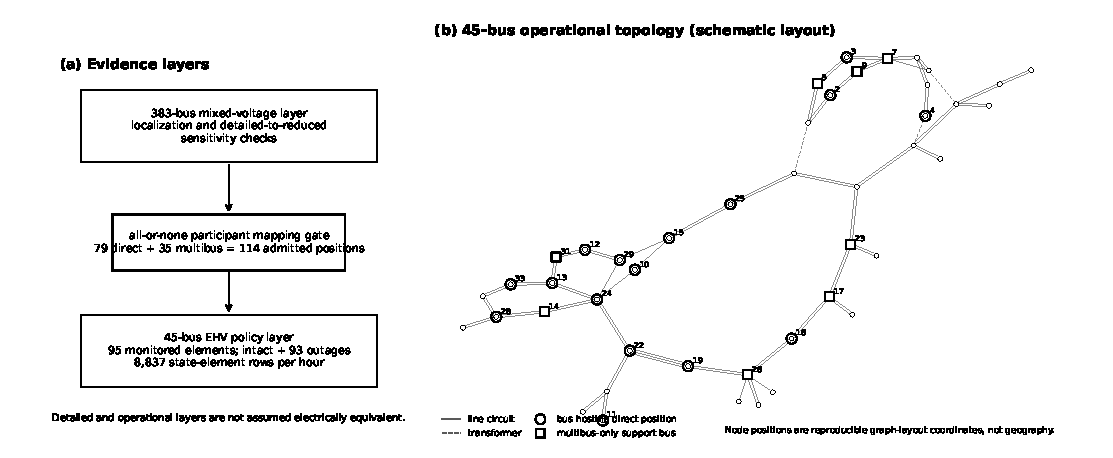
\includegraphics[width=0.99\linewidth]{dutch_case_architecture.pdf}
\caption{Dutch study architecture and schematic operational topology. The 383-bus structural layer informs localization and aggregation checks; the 45-bus layer is used for optimization. Circles denote buses hosting direct positions and squares additional multibus support buses. The diagram is schematic, not geographical.}
\label{fig:dutch}
\end{figure}

\begin{table}[ht]
\centering\small
\caption{Reported residuals in millions of MW$\cdot$h$\cdot$row-state: M2 is raw rolling replay, $U$ and $C$ are guarded annual witnesses from rolling trajectories, and EC is a retrospective energy-capped witness.}
\begin{tabular}{@{}crrrr@{}}\toprule
Year & M2 rolling & Uniform premium & Relief premium & Energy-capped relief\\\midrule
2028 & --- &155.100635&146.475468&152.760350\\
2029 &100.252003&120.434609&103.924090&110.550679\\
2030 &75.429906&92.851314&78.051920&84.367073\\
2031 &66.156571&81.395195&68.440753&73.450124\\\bottomrule
\end{tabular}
\end{table}
For 2029--2031, $100(S_U-S_C)/S_U$ gives 13.71\%, 15.94\%, and 15.92\%. The alternative $(S_U-S_C)/(S_U-S_{M2})$ gives 81.8\%, 84.9\%, and 85.0\% recovery of the observed uniform-to-M2 gap. Neither denominator defines a matched-exposure or causal effect.

The energy-capped residual improvements relative to the uniform control are 8.21\%, 9.14\%, and 9.76\% in 2029--2031. Each witness is feasible under both premium domains; the result therefore does not discriminate their annual feasible-set potential. Nor can the selected AC study be used to claim that the more favorable DC schedule is thermally secure.

\section{Interpretation and model boundaries}
The inclusions, hybrid projection, and dual inequalities hold for the stated model. New exported multipliers support independent guarded lower endpoints without changing the historical archive; no complete interval enclosure is claimed. Feasible depth actions, carried balances, and full-row objectives were replayed. The 18-hour AC sample excludes premiums. Actuator floors, critical-row PTDF errors, feasible balancing, matched premium AC cases, and forecast-vintage policies address different operational questions; annual soft-thermal residuals do not resolve them.

\section*{Acknowledgment}
OpenAI ChatGPT assisted with drafting and editing Sections 1--9; OpenAI Codex assisted with verification-code development and numerical checks \cite{OpenAI2026}. The authors retain responsibility for final verification and approval of the mathematics, data, and interpretation.
\bibliographystyle{IEEEtranN}
\bibliography{references}
\end{document}
